\documentclass[11pt,pointlessnumbers,DIV10,BCOR10mm,tocleft]{scrreprt}
\setcounter{tocdepth}{2} 
%\typearea[5mm]{13}

% --- ALLGEMEINES; EINGABE; ZEICHEN ---
%\usepackage[T1]{fontenc}
\usepackage[utf8]{inputenc}
\usepackage[ngerman]{babel}
\usepackage{amssymb,amsmath,amsfonts,stmaryrd}
\usepackage{wasysym,relsize}

% --- INDEX ---
\usepackage{makeidx}
\makeindex

% --- DIVERSES ---
\usepackage{graphicx}
\usepackage{enumerate}


% --- FARBEN UND PSTRICKS ---
\usepackage{color,pstricks}
\newgray{gray}{0.25}
\newgray{komagray}{0.4}
\newgray{lightgray}{0.45}
\newgray{verylightgray}{0.65}
\newgray{verydarkgray}{0.15}
\newrgbcolor{green}{0 0.75 0}

% --- TITELFARBEN ---
\newrgbcolor{screenblue} {0.588 0.667 0.745}
\newrgbcolor{Screenblue} {0.275 0.431 0.667}
\newrgbcolor{dekoblue}   {0.392 0.588 0.863}
\newrgbcolor{screenbrown}{0.851 0.851 0.816}
\newrgbcolor{Screenbrown}{0.824 0.824 0.784}
\newrgbcolor{SCREENBROWN}{0.745 0.745 0.725}
\newrgbcolor{dekobrown}  {0.686 0.686 0.667}
\newrgbcolor{Dekobrown}  {0.667 0.667 0.647}
\newrgbcolor{printcolor} {0.195 0.195 0.195}

% --- KOMA-ANPASSUNGEN ---
\newgray{komagray}{0.4}
\addtokomafont{sectioning}{\komagray}
\setkomafont{pagehead}{\normalfont\komagray\large\sffamily}
\addtokomafont{pagenumber}{\usekomafont{pagehead}}
\addtokomafont{footnote}{\komagray}

% --- ANPASSUNGEN ---
\renewcommand{\labelitemi}{$\circ$}
\renewcommand{\labelenumi}{(\arabic{enumi})}
\renewcommand{\labelenumii}{(\roman{enumii})}
\renewcommand{\labelenumiii}{(\alph{enumiii})}
% --- LAENGEN-ANPASSUNGEN ---
\setlength{\parindent}{0pt}
\setlength{\parskip}{1.6ex plus 0.2ex minus 0.2ex}
\psset{unit=1cm}
 % pakete laden, werte einstellen
%inhaltszähler
\newcounter{content}[chapter]
\newcounter{subcontent}[content]

%inhaltstyp
\newcommand{\contenttype}[2]{%
\stepcounter{content}%
\subsection*{#2 \thechapter.\thecontent: #1}%
\addcontentsline{toc}{subsection}{\numberline{}#2 \thechapter.\thecontent: #1}}

% inhalte
\newcommand{\definition}[1]{\contenttype{#1}{Definition}}
\newcommand{\proposition}[1]{\contenttype{#1}{Proposition}}
\newcommand{\lemma}[1]{\contenttype{#1}{Lemma}}
\newcommand{\korollar}[1]{\contenttype{#1}{Korollar}}
\newcommand{\satz}[1]{\contenttype{#1}{Satz}}
\newcommand{\folgerung}[1]{\contenttype{#1}{Folgerung}}
\newcommand{\beispiel}[1]{\contenttype{#1}{Beispiel}}


%unterinhaltstyp
\newcommand{\subcontenttype}[2]{%
\stepcounter{subcontent}%
\subsection*{#2 \thechapter.\thecontent.\alph{subcontent}: #1}%
\addcontentsline{toc}{subsection}{\numberline{}#2 \thechapter.\thecontent.\alph{subcontent}: #1}}

%subinhalte
\newcommand{\subdefinition}[1]{\subcontenttype{#1}{Definition}}
\newcommand{\subproposition}[1]{\subcontenttype{#1}{Proposition}}
\newcommand{\sublemma}[1]{\subcontenttype{#1}{Lemma}}
\newcommand{\subkorollar}[1]{\subcontenttype{#1}{Korollar}}
\newcommand{\subsatz}[1]{\subcontenttype{#1}{Satz}}
\newcommand{\subfolgerung}[1]{\subcontenttype{#1}{Folgerung}}
\newcommand{\subbeispiel}[1]{\subcontenttype{#1}{Beispiel}}


%weitere strukturen
\newcommand{\bsp}[1]{\subsubsection*{Beispiel: #1}}
\newcommand{\bsps}[1]{\subsubsection*{Beispiele: #1}}
\newcommand{\beweis}{\subsubsection*{Beweis:}}
\newcommand{\bemerkung}{\subsubsection*{Bemerkung:}}


%für aufgabenzettel und lösungen
\newcounter{series}
\newcounter{task}[series]

\newcommand{\series}{
\stepcounter{series}%
\section*{Serie \theseries}%
\addcontentsline{toc}{section}{\numberline{}{Serie \theseries}}}

\newcommand{\task}{\stepcounter{task}\subsection*{Aufgabe \thetask}\vspace{-2ex}\markright{Aufgabe \thetask}}
\newcommand{\solution}{\subsubsection*{Beweis:}}

   % eigene befehle
%mengen u.s.w
\newcommand{\pmenge}{\mathcal{P}}
\newcommand{\setN}{\mathbb{N}}
\newcommand{\setR}{\mathbb{R}}
\newcommand{\setQ}{\mathbb{Q}}
\newcommand{\setE}{\mathbb{E}}

% abkuerzuungen
\newcommand{\w}{\omega}

\newcommand{\wkeit}{\ensuremath{\,\mathbb{P}}}
\newcommand{\Wkeit}{Wahrscheinlichkeit{ }}

\newcommand{\wmas}{\ensuremath{\,\mathbb{P}}}
\newcommand{\Wmas}{Wahrscheinlichkeitsmaß{ }}

\newcommand{\wraum}{\ensuremath{(\varOmega, \varSigma, \mathbb{P})}{ }}
\newcommand{\Wraum}{Wahrscheinlichkeitsraum{ }}

%operatoren 
\newcommand{\var}{\mathrm{\,Var}}
\newcommand{\cov}{\mathrm{\,Cov}}
\newcommand{\vol}{\mathrm{\,Vol}}
\newcommand{\ber}{\mathrm{\,Ber}}
\newcommand{\bin}{\mathrm{\,Bin}}
\newcommand{\geom}{\mathrm{\,Geom}}
\newcommand{\poi}{\mathrm{\,Poi}}

%große operatoren mit \limits
\newcommand{\Int}{\textstyle\int\limits}
\newcommand{\Sum}{\textstyle\sum\limits}
\newcommand{\Prod}{\textstyle\prod\limits}
\renewcommand{\Cup}{\textstyle\bigcup\limits}
\renewcommand{\Cap}{\textstyle\bigcap\limits}

%deutsche anführungszzeichen
\newcommand{\gqq}[1]{\glqq{#1\grqq}}
\newcommand{\gq}[1]{\glq{#1\grq}}   % eigene mathe-befehle

\renewcommand{\thesection}{\arabic{section}}
\renewcommand{\thefigure}{\arabic{figure}}

\begin{document}
% --- TITEL ---

% --- SCHMUTZTITEL ---
\cleardoublepage
\verydarkgray
\chapter*{Software-Challenge 2011}
\vspace*{-.9cm}
\section*{Dokumentation zum Spielserver der Software-Challenge}
\pagenumbering{arabic}
\thispagestyle{empty}
\vspace*{-.2cm}
\vfill
Stand: \today

% --- INHALTSVERZEICHNISS ---
\pagestyle{headings}
\tableofcontents

\pagestyle{plain}
\stepcounter{chapter}
\chapter*{Spielserver und Clients}

\section{Programmoberfläche}
Die Programmoberfläche besteht aus dem Menü, der Spielfläche und der Statusleiste.

Über das Menü oben sind alle Funktionen des Servers erreichbar. Die Spielfläche in der Mitte
mit den Steuerelementen dient zur Anzeige der Spiele. Die Statusleiste unten gibt kurze
Statusinformationen zum Spiel aus.

Zu Beginn ist die Spielfläche leer.

\section{Ein neues Spiel erstellen}
Um ein Spiel zu spielen, muss zunächst über das Menü \glqq{Spiel\grqq} $\to$ \glqq{Neues Spiel erstellen\grqq} das
in Abbildung \ref{neuesspiel} gezeigte Menü aufgerufen werden.

\begin{figure}
 \centering
 \newsavebox\NEUESMENUE
 \sbox\NEUESMENUE{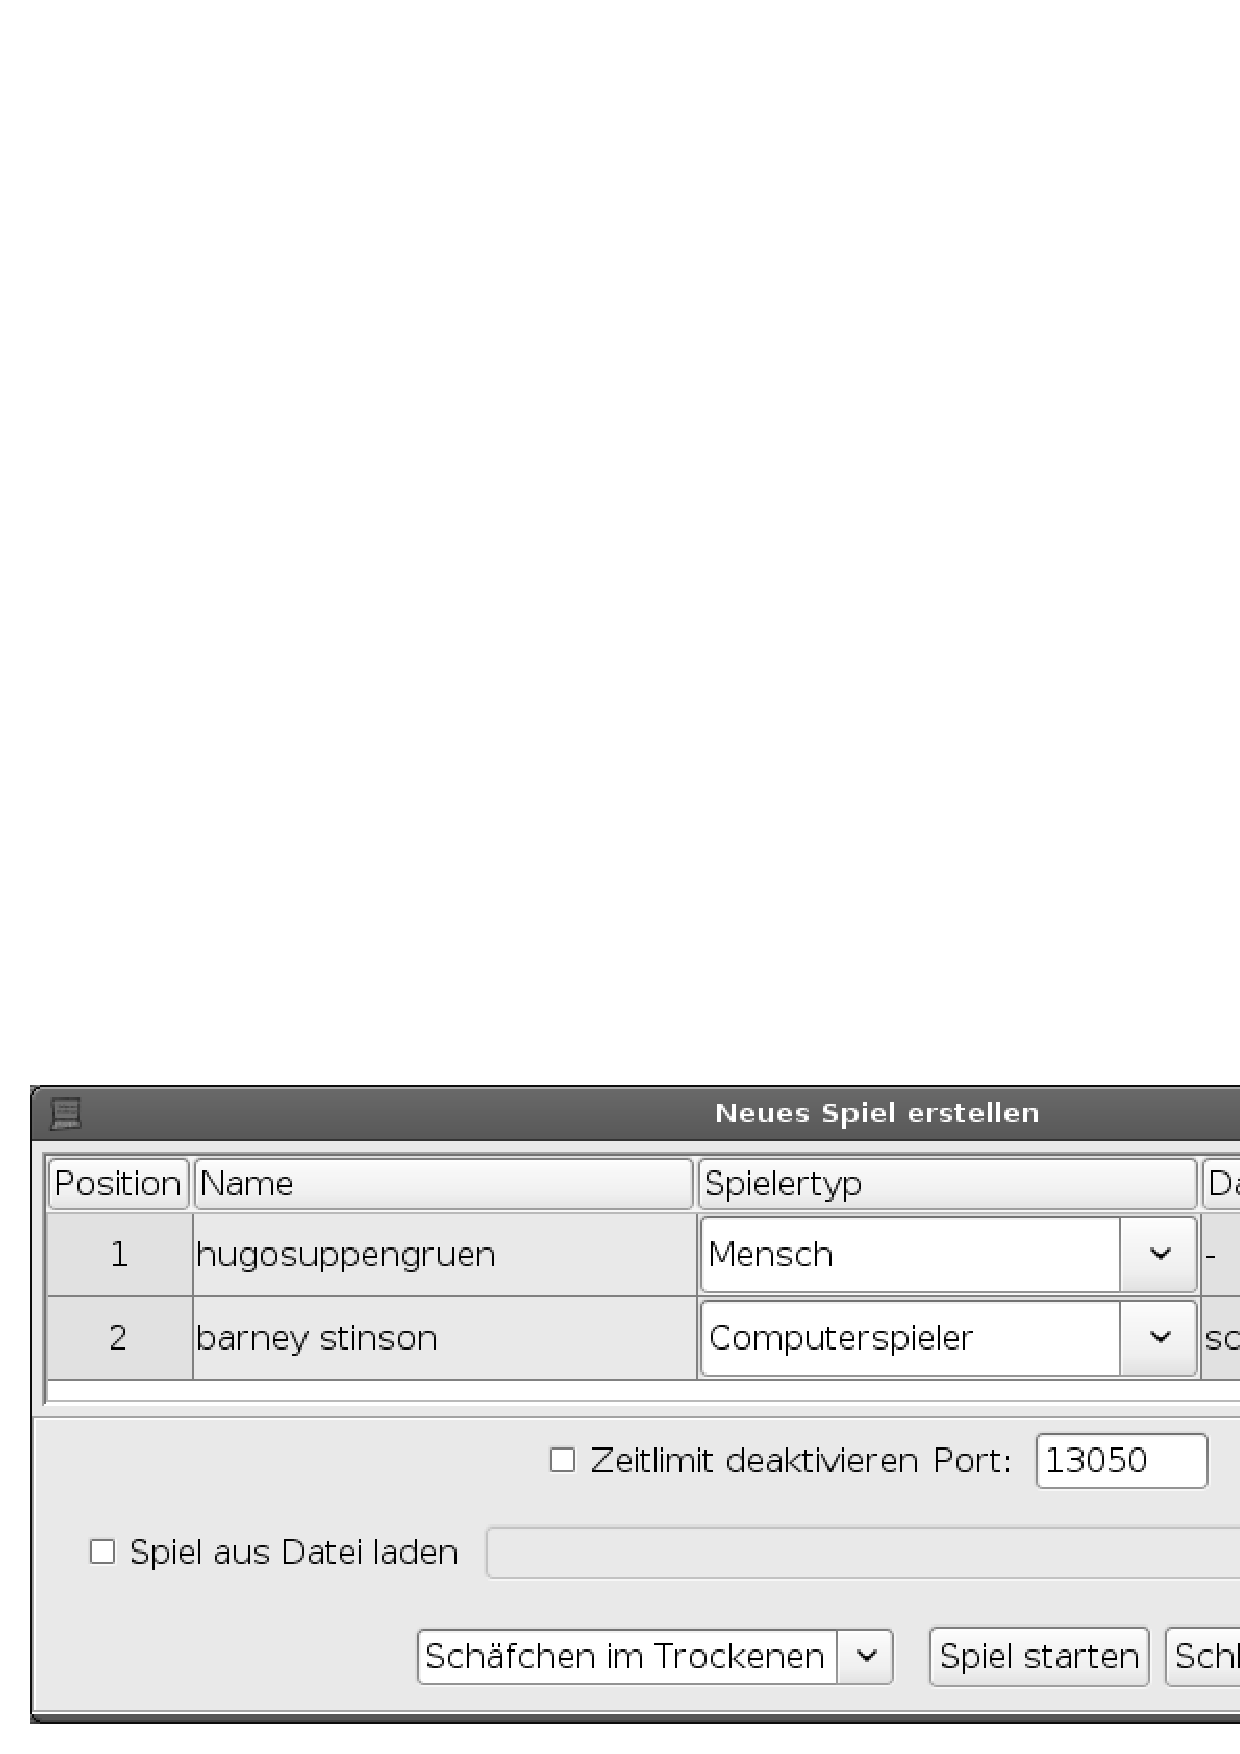
\includegraphics[scale=0.45]{ps/neuesspiel}}%
 \begin{pspicture}[showgrid=false](0,0)(\wd\NEUESMENUE,\ht\NEUESMENUE)
  \rput[lb](0,0){\usebox\NEUESMENUE}
 \end{pspicture}
 \caption{Ein neues Spiel erstellen.}\label{neuesspiel}
\end{figure}

In diesem Fenster werden die Spieler ausgewählt, die an dem Spiel teilnehmen sollen.
Die vier Spalten sind folgendermaßen zu verstehen:

\begin{itemize}
\item \textbf{Position:} Stellt die Startpositionen der einzelnen Spieler dar. Der Spieler an Position Eins beginnt.
\item \textbf{Name:} Hier kann für jeden Spieler ein Name eingegeben werden, der dann im Spiel angezeigt wird.
\item \textbf{Spielertyp} Es kann zwischen 3 verschiedenen Spielertypen gewählt werden:
\begin{itemize}
\item \textbf{Mensch:} Ein menschlicher Spieler, der über die Programmoberfläche spielt.
\item \textbf{Computerspieler:}  Ein Computerspieler in Form eines separaten Programms, das beim Starten des Spiels automatisch vom Server gestartet wird.
\item \textbf{Computerspieler (manuell):}  Ein Computerspieler in Form eines separaten Programms, das manuell durch den Benutzer gestartet werden muss.
\end{itemize}
\item \textbf{Dateiname:} Bei Spielertyp \glqq{Computerspieler\grqq} ist eine Programmdatei auszuwählen, deren Name dann hier angezeigt wird. Bei anderen
Spielertypen wird dort \glqq{--\grqq} angezeigt.
\end{itemize}

Unten lässt sich der Port für das Spiel einstellen. Dieser wird zum Verbinden der Programme
mit dem Server benötigt, insbesondere für diejenigen, die manuell gestartet werden.
Standardmäßig ist 13050 eingestellt.

Links daneben kann wahlweise das Zeitlimit für einen Zug für Computerspieler deaktiviert
werden. Menschliche Spieler können immer unbeschränkt lange über ihren aktuellen Zug
nachdenken. Das Zeitlimit ist abhängig vom ausgewählten Spieltyp (s.u. und entsprechende
Dokumentation). Benötigt ein Computerspieler mehr Zeit für die Kalkulation eines Zuges,
wird das Spiel automatisch vom Server beendet und der Computerspieler verliert das Spiel.

Links unten kann der Spieltyp ausgewählt werden, insbesondere das aktuelle Spiel der Software-Challenge.

Nach Eingabe der erforderlichen Werte kann das Spiel mithilfe des unteren Buttons \glqq{Spiel
starten\grqq} erstellt werden. Dabei erscheint der Dialog \glqq{Warte auf Spieler...\grqq\ solange, bis alle
Computerspieler gestartet und mit dem Server verbunden wurden.

Es kann immer nur höchstens ein Spiel zurzeit über den Server gespielt werden.

\section{Spielfeldoberfläche}
Die Spielfeldoberfläche setzt sich aus dem eigentlichen Spielbrett und den in Abbildung \ref{steuerelemente} gezeigen Steuerelementen zusammen. 

Auf dem Spielbrett werden das eigentliche Spiel, die Züge und weitere für das Spiel wichtige Informationen dargestellt. Hier setzt der menschliche Spieler
auch seine Züge.

\begin{figure}
 \centering
 \newsavebox\STEUERELEMENTE
 \sbox\STEUERELEMENTE{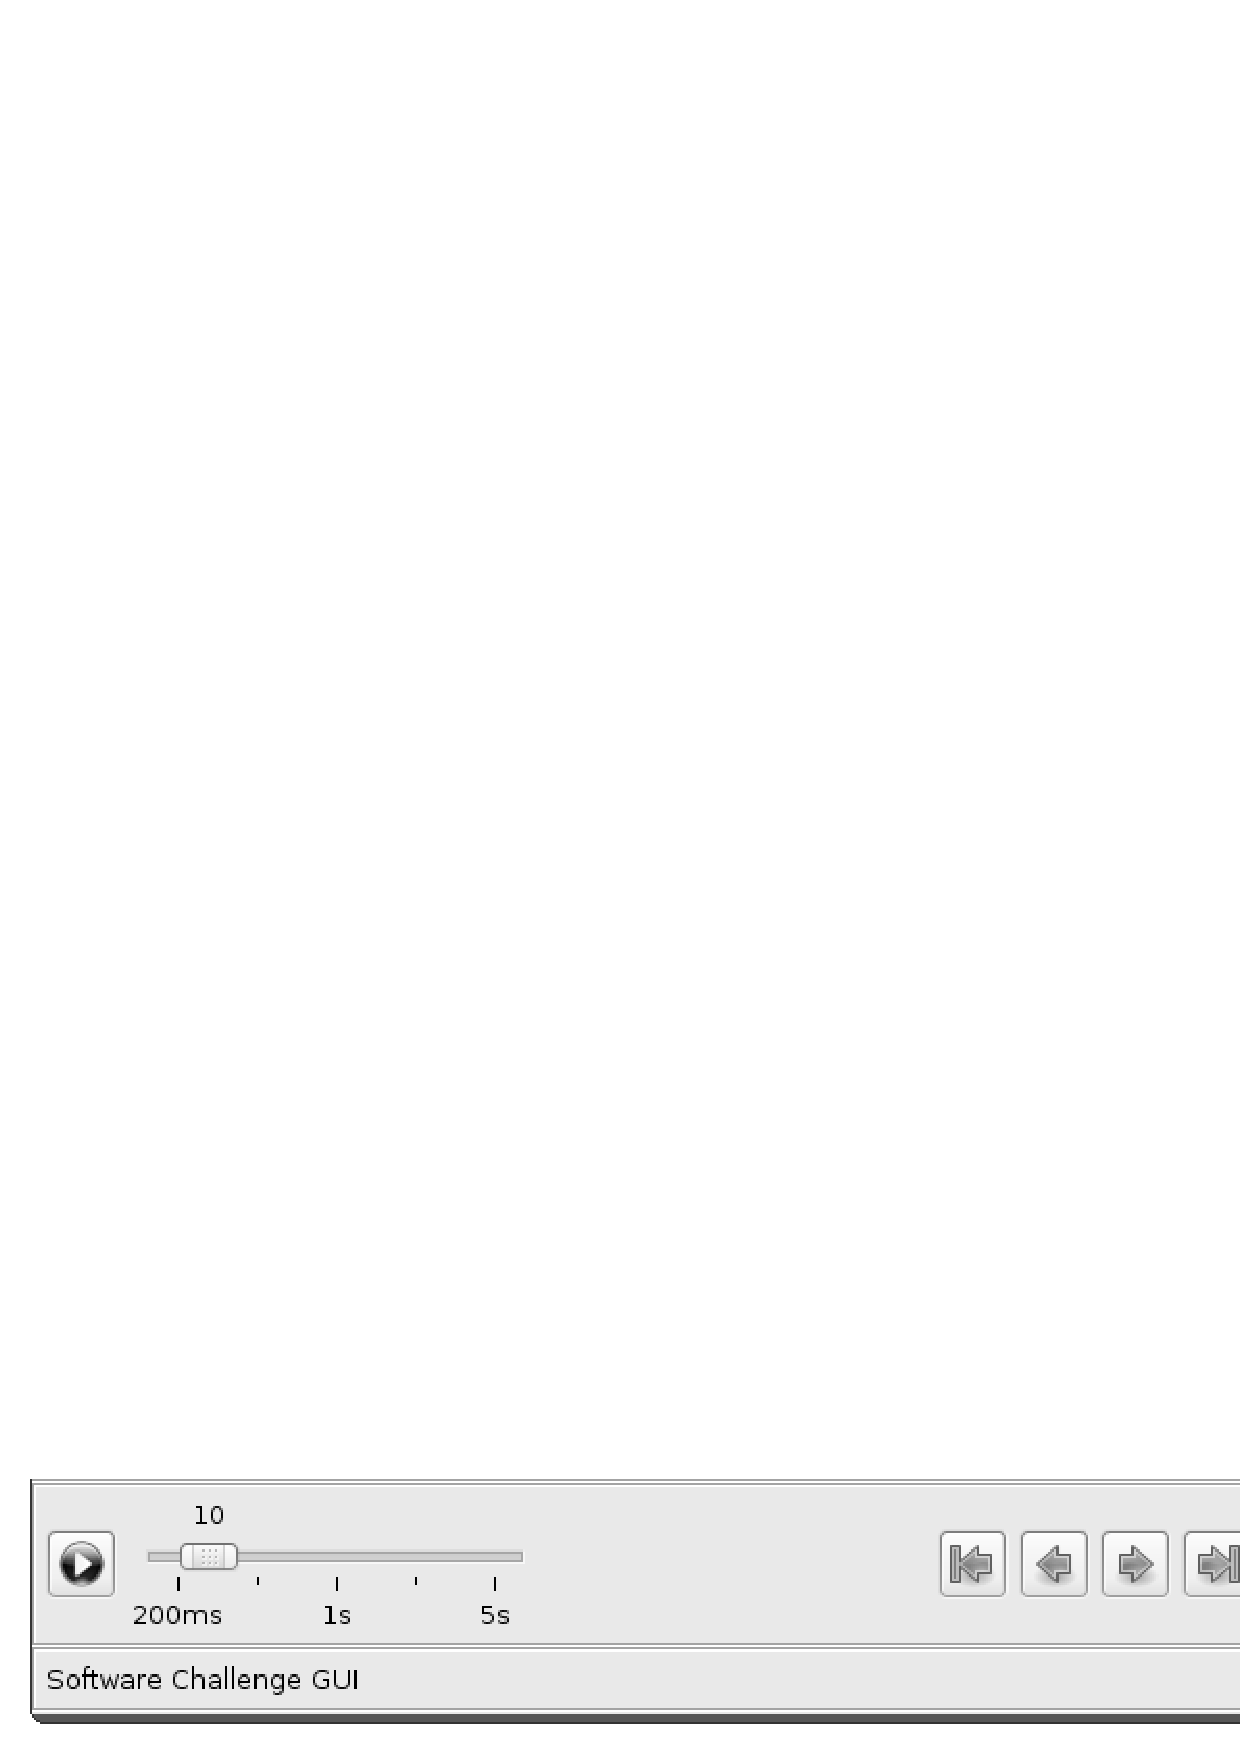
\includegraphics[scale=0.375]{ps/steuerelemente}}%
 \begin{pspicture}[showgrid=false](0,0)(\wd\STEUERELEMENTE,\ht\STEUERELEMENTE)
  \rput[lb](0,0){\usebox\STEUERELEMENTE}
  \rput(.33,1.65){\pscircle[fillstyle=solid,fillcolor=red,linestyle=none]{0.25}\rput[B](-.01,-.1){\white a}}
  \rput(6,1.65){\pscircle[fillstyle=solid,fillcolor=red,linestyle=none]{0.25}\rput[B](-.01,-.1){\white b}}
  \rput(6.5,1.65){\pscircle[fillstyle=solid,fillcolor=red,linestyle=none]{0.25}\rput[B](-.01,-.1){\white c}}
  \rput(7,1.65){\pscircle[fillstyle=solid,fillcolor=red,linestyle=none]{0.25}\rput[B](-.01,-.1){\white d}}
  \rput(7.5,1.65){\pscircle[fillstyle=solid,fillcolor=red,linestyle=none]{0.25}\rput[B](-.01,-.1){\white e}}
  \rput(13.2,1.65){\pscircle[fillstyle=solid,fillcolor=red,linestyle=none]{0.25}\rput[B](-.01,-.1){\white f}}
 \end{pspicture}
 \caption{Die Steuerelemente, a) Spiel starten, b) zum Anfang, c) einen Schritt zurück, d) einen Schritt weiter, e) zum Ende, f) Spiel abbrechen.}\label{steuerelemente}
\end{figure}

Der \glqq{Spiel starten\grqq}-Button muss nicht zwingen betätigt werden. Mit den Steuerelementen kann man sich den bisherigen Spielverlauf angucken. Wenn wenigstens ein Computerspieler mitspielt muss man den \glqq{Einen Schritt weiter\grqq}-Button betätigen um den Zug des Computerspielers anzufordern. Alternativ kann man durch betätigen des \glqq{Spiel starten\grqq}-Buttons dafür sorgen, dass die Züge des Computerspielers automatisch angefordert werden.

\section{Spielwiederholung laden}
Nachdem ein Spiel beendet wurde, sei es durch den Benutzer, aufgrund der Spielregeln oder
aus einem anderen Grund, wird eine Wiederholungsdatei im Ordner \glqq{replay\grqq} erstellt. Diese
kann über das obige Menü unter \glqq{Spiel\grqq} $\to$ \glqq{Spielwiederholung laden\grqq} ausgewählt werden.
Dabei öffnet sich das in Abbildung \ref{wiederholung} gezeigte Fenster.

\begin{figure}
 \centering
 \newsavebox\WIEDERHOLUNG
 \sbox\WIEDERHOLUNG{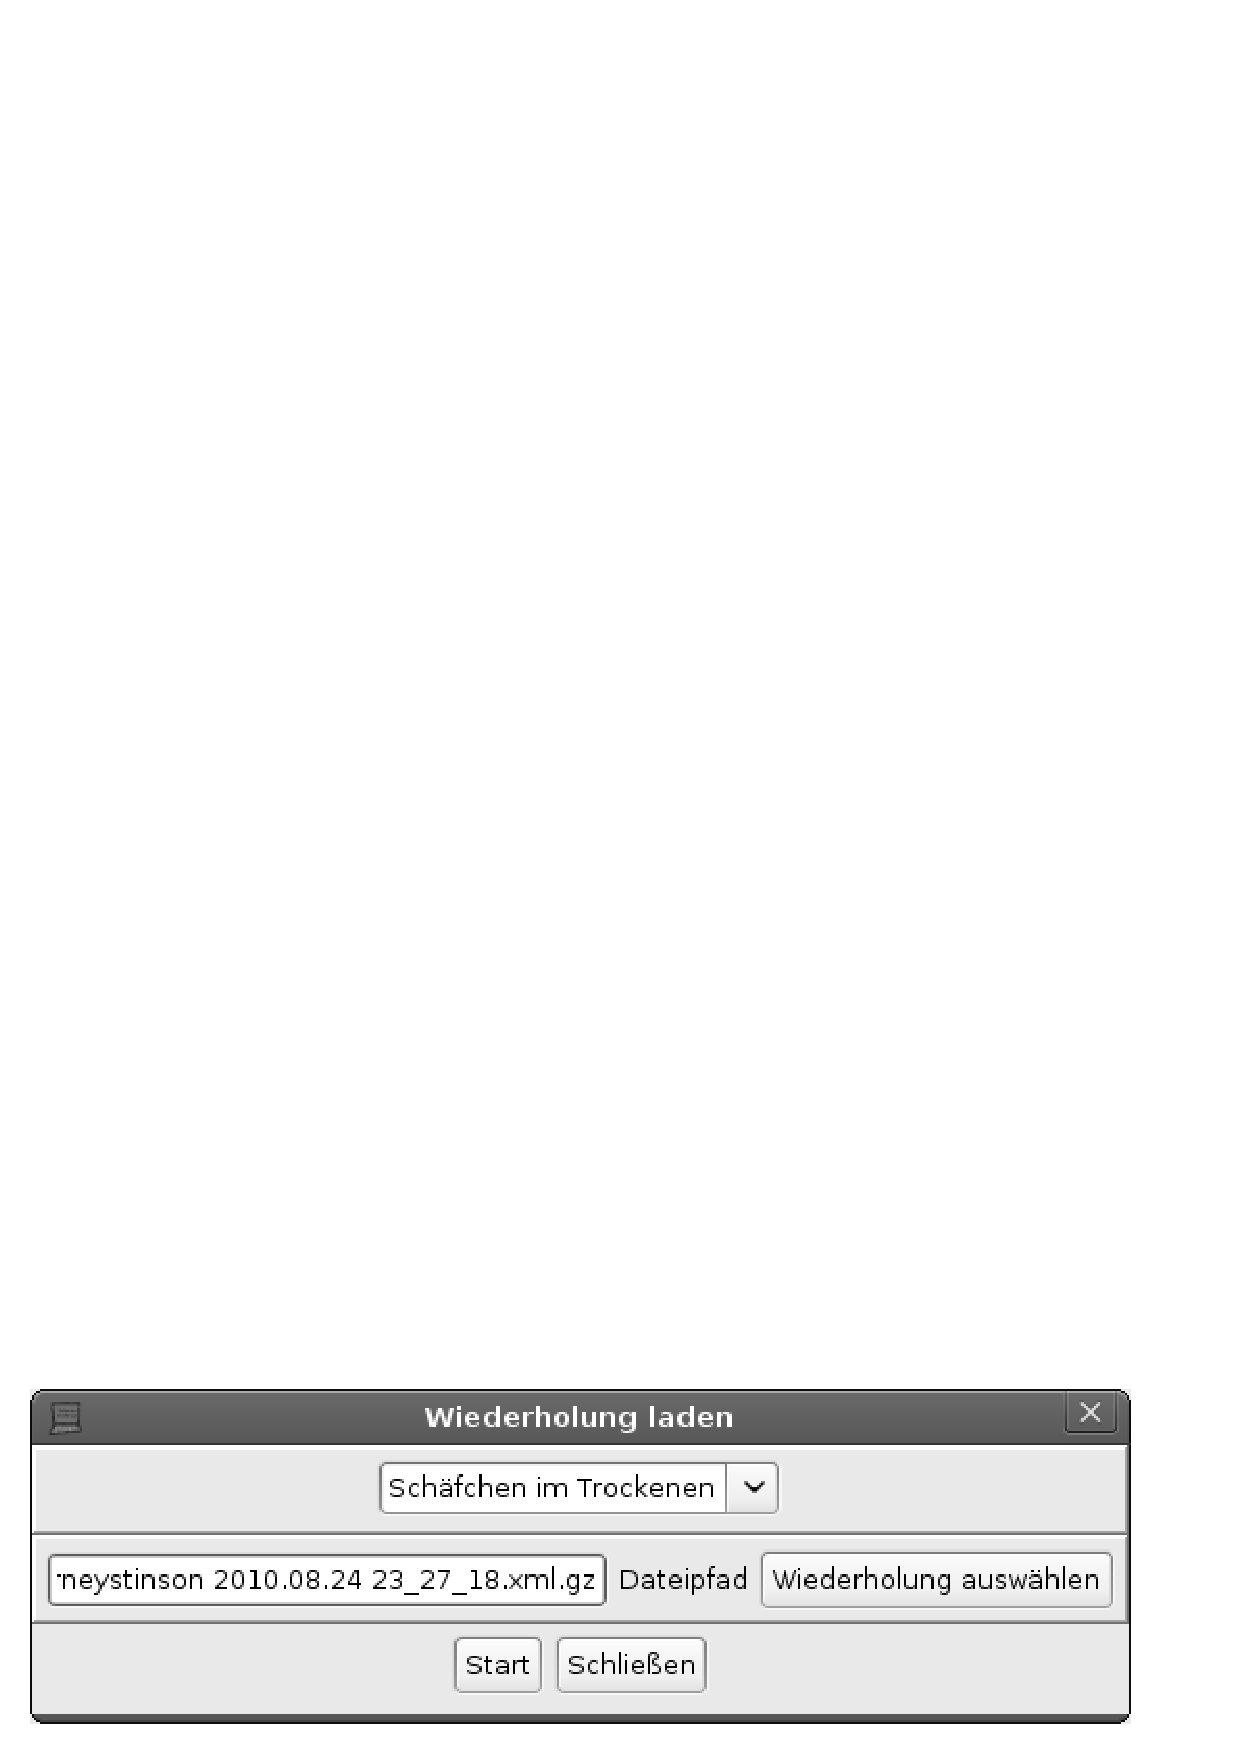
\includegraphics[scale=0.45]{ps/wiederholung}}%
 \begin{pspicture}[showgrid=false](0,0)(\wd\WIEDERHOLUNG,\ht\WIEDERHOLUNG)
  \rput[lb](0,0){\usebox\WIEDERHOLUNG}
 \end{pspicture}
 \caption{Spielwiederholung laden.}\label{wiederholung}
\end{figure}

Oben muss der Spieltyp der zu ladenden Wiederholung ausgewählt werden.

Nach Betätigung des Knopfes \glqq{Wiederholung auswählenßgrqq} kann die Replay-Datei des
gewünschten Spiels gewählt werden. Die Dateinamen sind dabei nach folgendem Schema
aufgebaut, wobei anstelle der kursiven Worte die Werte des betreffenden Spiels einzusetzen
sind:

\begin{center}
replay\_\textit{Spielername1}\_\textit{Spielername2} \textit{Datum} \textit{Uhrzeit}.xml.gz
\end{center}
Z.B. also \glqq{replay\_hugosuppengruen\_barneystinson 2010.08.24 23\_27\_18.xml.gz\grqq}.

Betätigen des \glqq{Spiel starten\grqq}-Buttons dafür sorgen, dass das Raplay automatisch abgespielt wird. Alternativ kann man auch mit den anderen Steuerelementen durch das Replay navigieren.

\section{Testdurchläufe}
Über das Menü \glqq{Spiel\grqq} $\to$ \glqq{Testdurchläufe\grqq} gelangt man zum in Abbildung \ref{testdurchlaeufe} gezeigtem Fenster. Hier kann man Computerspieler (keine menschlichen Spieler) gegeneinander in mehreren Spielen hintereinander antreten lassen und erhält eine ausführliche
Statistik über die absolvierten Spiele.

\begin{figure}
 \centering
 \newsavebox\TESTDURCHLAEUFE
 \sbox\TESTDURCHLAEUFE{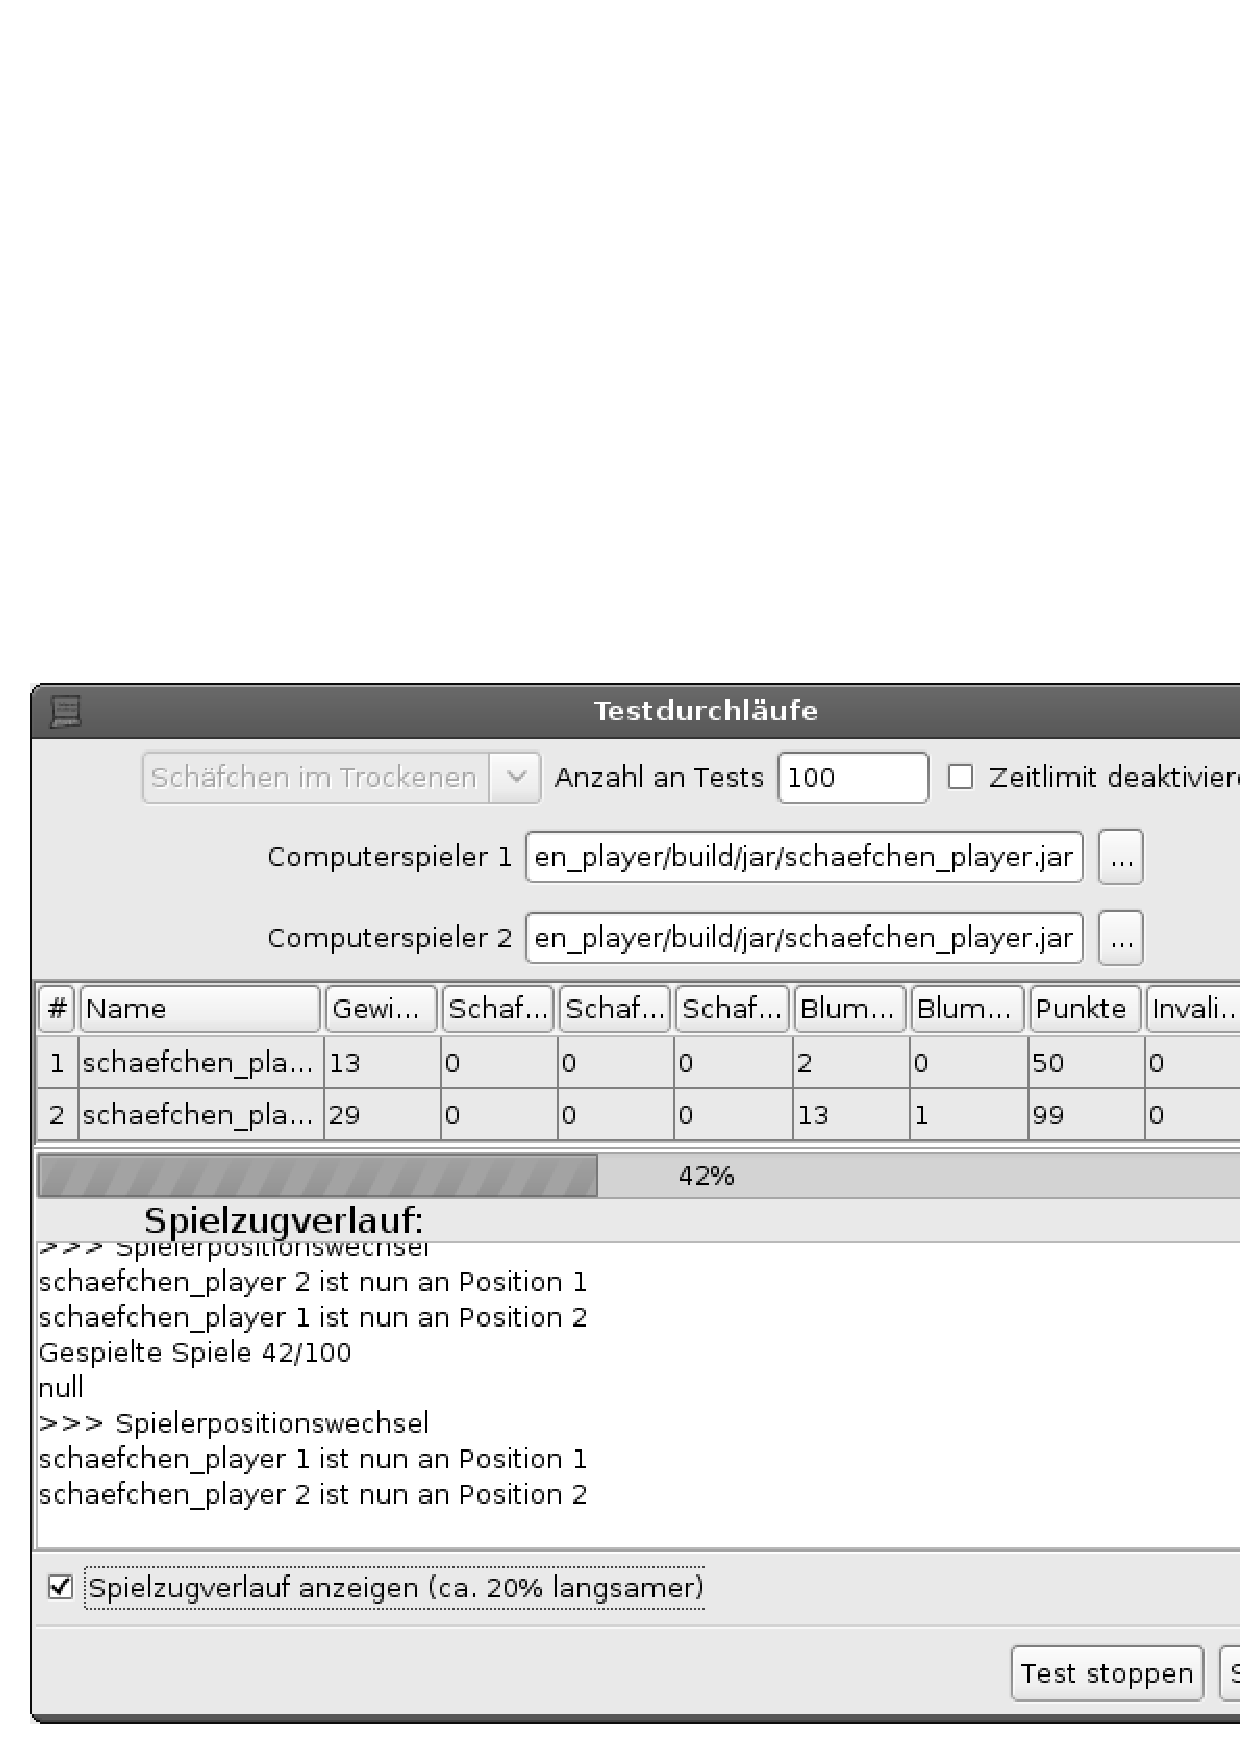
\includegraphics[scale=0.45]{ps/testdurchlaeufe}}%
 \begin{pspicture}[showgrid=false](0,0)(\wd\TESTDURCHLAEUFE,\ht\TESTDURCHLAEUFE)
  \rput[lb](0,0){\usebox\TESTDURCHLAEUFE}
 \end{pspicture}
 \caption{Spielwiederholung laden.}\label{testdurchlaeufe}
\end{figure}

Oben muss der Spieltyp ausgewählt, rechts daneben die Anzahl der Spiele eingegeben
werden. Außerdem kann wieder optional das Zeitlimit deaktiviert werden.

Darunter sind die Computerspieler auszuwählen. Anschließend kann der Test durch das
Anklicken des entsprechenden Knopfes unten rechts gestartet werden.

Sollte es während der Testdurchläufe zu einem fehlerhaften Spiel kommen, wird dieses als
Replay-Datei gespeichert. Andere Spiele werden nicht gespeichert.


%\chapter{Mit dem Server kommunizieren}



\end{document}


